\chapter{Integration and Differentiation} \label{ch:intdiff}

Many functions are simple to integrate or differentiate by hand. You know the basic rules for trigonmetric functions, logs, exponentials, polynomials. But in some complicated (sometimes real-world) applications you may need to integrate or differentiate a function that has no closed-form expression. In this chapter we develop numerical methods to deal with these kinds of problems.

\section{Numerical integration}
The goal is to integrate some known function, $f(x)$, over an interval $[a,b]$, giving just 1 real value
\begin{align*}
I = \int_a^b f(x) dx.
\end{align*}
That is, the find the area under its curve, as graphed in figure~\ref{fig:ch5_integration}.

\begin{figure}[H]
	\begin{center}
	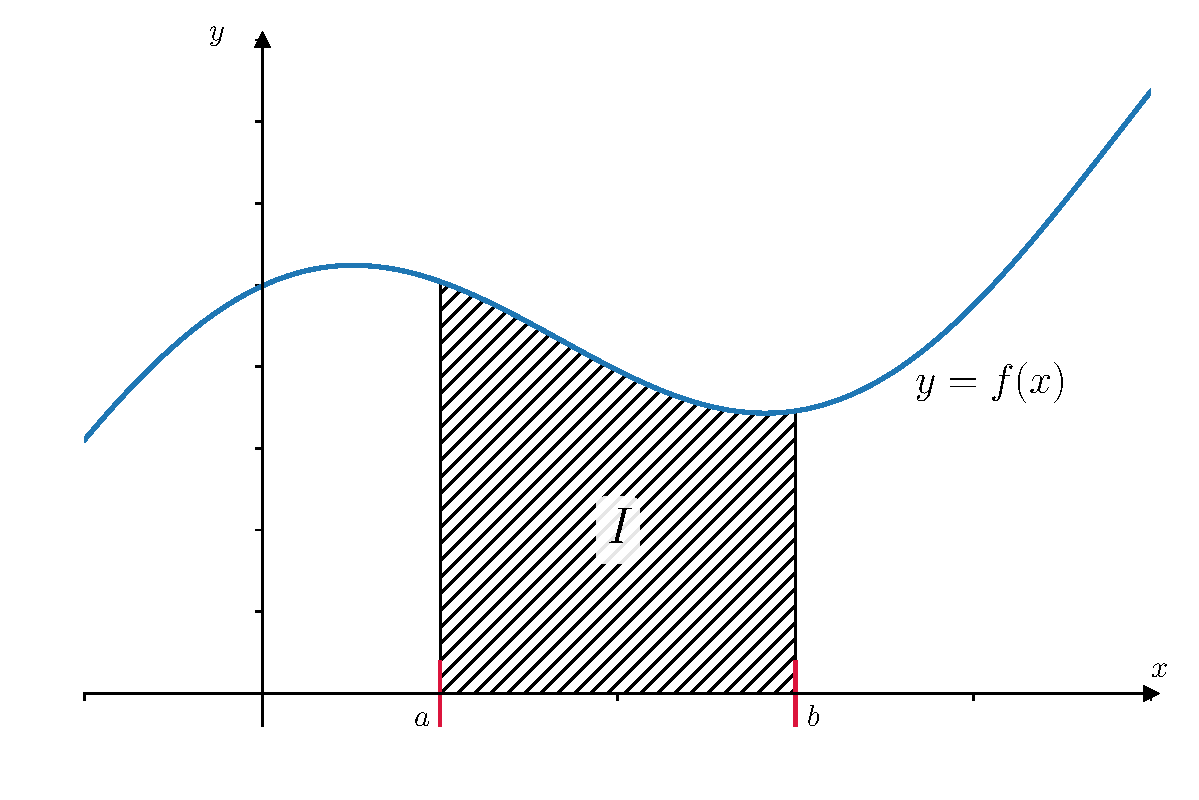
\includegraphics[width=0.6\textwidth]{figures/ch5_integration.pdf} 
	  \caption{.} \label{fig:ch5_integration}
	\end{center}
\end{figure}

The method we will use is to first estimate $f(x)$ with the Lagrangian interpolation polynomial, $p_n(x)$, and integrate that instead. So we have the approximation for the integral
\begin{align*}
I \sim \int_a^b p_n(x) dx.
\end{align*}
Figure~\ref{fig:ch5_lagrangian} shows the general schema, where we interpolate $f(x)$ using $n+1$ evenly spaced points on $[a,b]$ (including the end points).
\begin{figure}[H]
	\begin{center}
	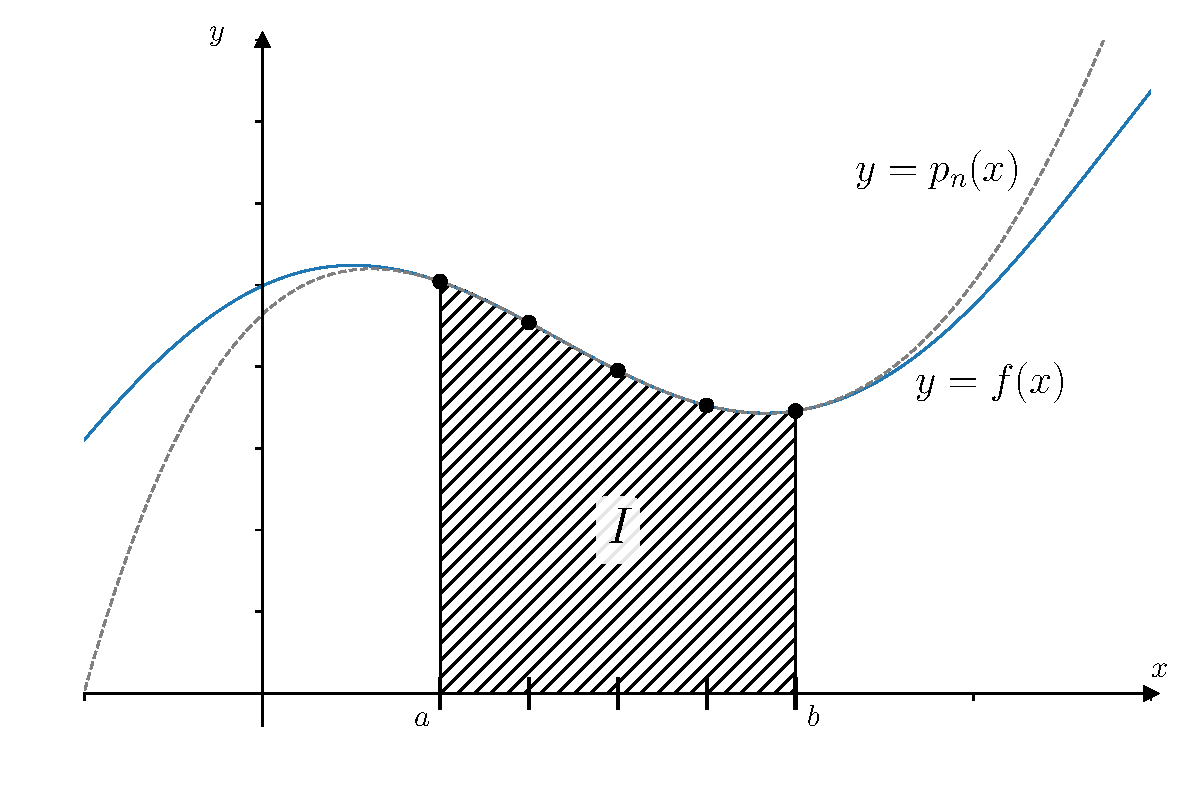
\includegraphics[width=0.6\textwidth]{figures/ch5_lagrangian.pdf} 
	  \caption{.} \label{fig:ch5_lagrangian}
	\end{center}
\end{figure}

Recall from Chapter~\ref{ch:polynomial} that the interpolation polynomial through $n+1$ points is given by a sum over the $y$ values of the interpolation points multiplied by Lagrange basis polynomials
\begin{align*}
p(x)  = \sum_{k=0}^n y_k L_k(x) = \sum_{k=0}^n y_k \prod_{i\neq k} \frac{x-x_i}{x_k-x_i}.
\end{align*}
Since the interpolation points are given by a known function, we can set $y_k=f(x_k)$. The even spacing on $[a,b]$ also gives us the expressions for the $x$ values of the interpolation points
\begin{align*}
x_k = a + k\frac{b-a}{n}, \quad k=0,1,2,\dots,n.
\end{align*}
So the integral is approximated by
\begin{align*}
I &\sim \int_a^b \sum_{k=0}^n f(x_k) L_k(x) dx \\
&=  \sum_{k=0}^n f(x_k) \int_a^b L_k(x) dx \\
&=  \sum_{k=0}^n f(x_k) w_k
\end{align*}
where we have introduced the ``quadrature weights''
\begin{align*}
w_k = \int_a^b L_k(x) dx.
\end{align*}
This formalism of approximating an integral with evenly spaced interpolation points gives a family of formulae for different number of interpolation points, $n+1$, called \textit{Newton-Cotes formulae}. In this chapter we'll only look at $n=1$ and $n=2$, which give rise to the Trapezium and Simpson's rules, respectively.

\subsection{Trapezium rule}
If we choose $n=1$, then we interpolate the function with $n+1=2$ points. These are merely the endpoints of the interval, $x_0=a$ and $x_1=b$. Interpolating with a polynomial of degree $n=1$ means a straight line connecting these two points. This integration approximation is graphed in figure~\ref{fig:ch5_trapezium}.
\begin{figure}[H]
	\begin{center}
	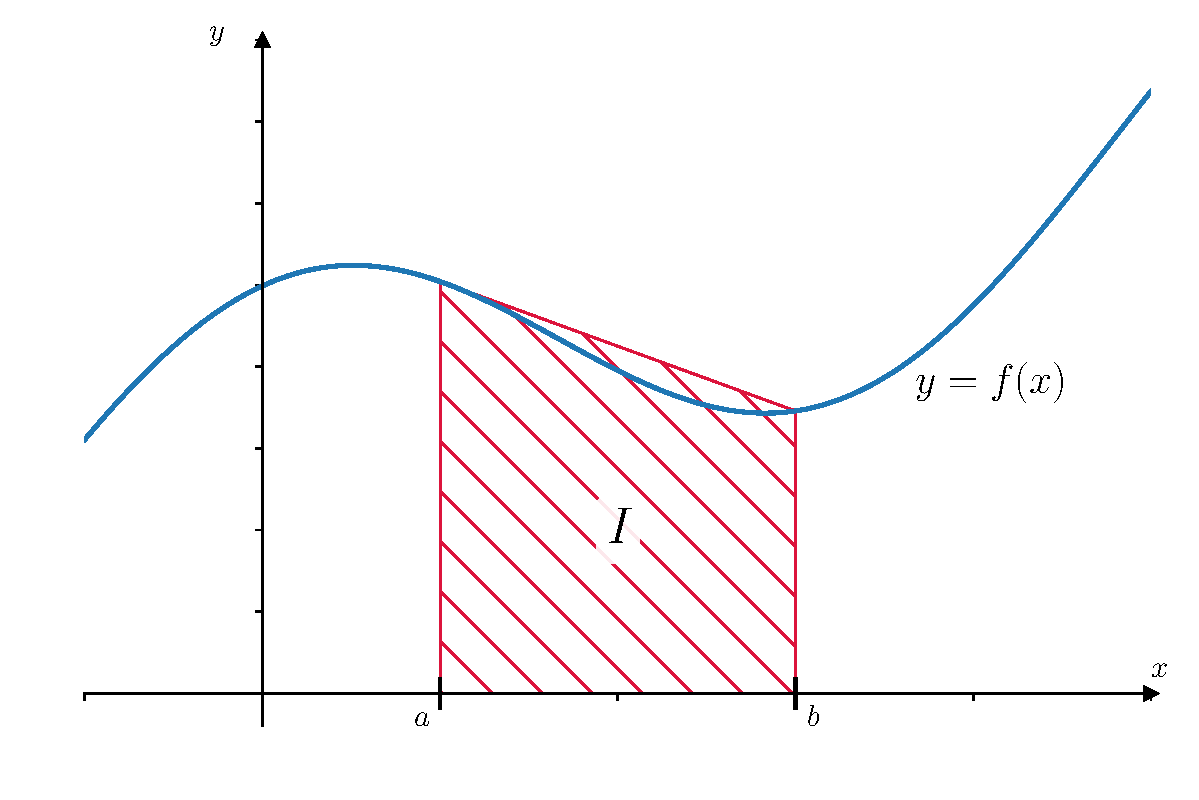
\includegraphics[width=0.6\textwidth]{figures/ch5_trapezium.pdf} 
	  \caption{.} \label{fig:ch5_trapezium}
	\end{center}
\end{figure}
The Newton-Cotes formula for $n=1$ is then
\begin{align*}
I \sim f(a) w_0 + f(b) w_1.
\end{align*}
Let's derive expressions for the quadrature weights. The zeroth weight is
\begin{align*}
w_0 &= \int_a^b L_0(x) dx, \quad \text{and } L_0 = \frac{x-b}{a-b} \\
 &= \frac{1}{a-b} \left. \left(\frac{x^2}{2} - bx \right) \right|_a^b \\
 &= \frac{1}{a-b} \left( -\frac{b^2}{2} - \frac{a^2}{2} + ba \right) \\
 &= -\frac{1}{2(a-b)} \left( a^2 - 2ab + b^2 \right) \\
 &= -\frac{1}{2(a-b)} \left( a - b \right)^2 \\
 &= \frac{b - a}{2}
\end{align*}
and similarly the first weight is
\begin{align*}
w_1 &= \int_a^b L_1(x) dx, \quad \text{and } L_1 = \frac{x-a}{b-a} \\
 &= \frac{1}{b-a} \left. \left(\frac{x^2}{2} - ax \right) \right|_a^b \\exercice
 &= \frac{1}{2(b-a)} \left( b - a \right)^2 \\
 &= \frac{b - a}{2}.
\end{align*}
The two weights are the same! Hence we have 

\noindent \fbox{\begin{minipage}{\linewidth}
\underline{\textbf{Trapezium rule for approximating an integral}}
\begin{align}
\int_a^b f(x)dx \sim \frac{b-a}{2}\left(f(a) + f(b) \right) 
\end{align}
\end{minipage}}

With a small rearrangement we can get an alternative geometric interpretation of this rule
\begin{align*}
I \sim \underbrace{\frac{f(a) + f(b)}{2}}_\text{average height in the range} \overbrace{\left(b-a \right)}^\text{size of range}.
\end{align*}
This is simply the formula for the area of the rectangle shown below, with height equal to the average height of the function in the integration interval $[a,b]$.

\begin{figure}[H]
	\begin{center}
	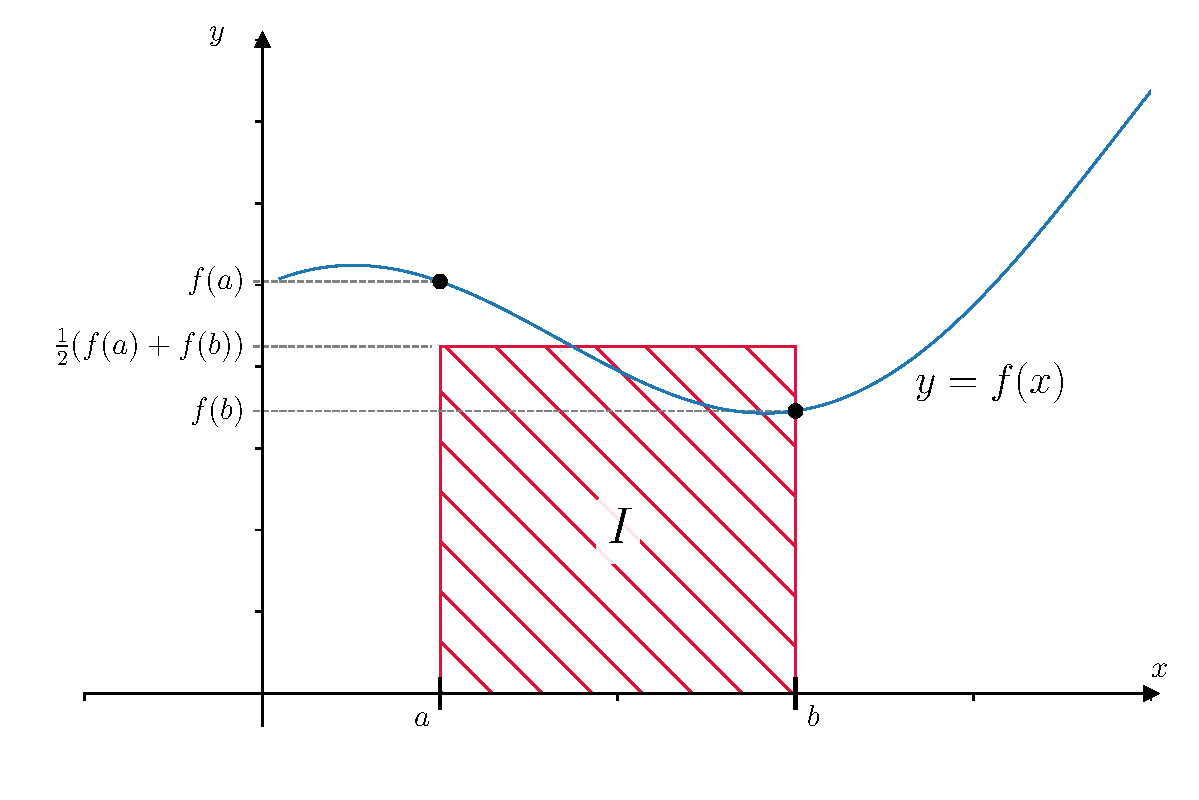
\includegraphics[width=0.6\textwidth]{figures/ch5_trapezium_alternative.pdf} 
	  \caption{.} \label{fig:ch5_trapezium_alternative}
	\end{center}
\end{figure}


%%%%%%%%%%%%%%%%%%%%%%%%%%%%%%%%%%%%%%%%%%%%%%%
%%%%%%%%%%% EXAMPLE TRAPEZIUM RULE %%%%%%%%%%%%
\exemple{\upline}
{
Integrate $f(x)=e^x$ from 0 to 4 using the Trapezium rule with two (equal-sized) subdivisions.

\noindent The two subdivisions are the intervals $[0,2]$ and $[2,4]$. The areas are sketched out below
\begin{figure}[H]
	\begin{center}
	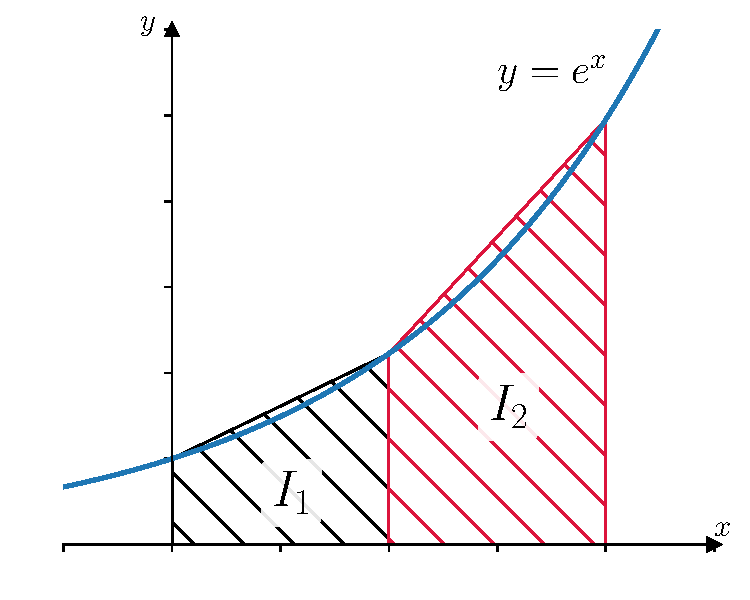
\includegraphics[width=0.6\textwidth]{figures/ch5_trapezium_example.pdf} 
	  \caption{.} \label{fig:ch5_trapezium_example}
	\end{center}
\end{figure}
The two integrals are then
\begin{align*}
&\int_0^2 e^x dx \sim I_1 = \frac{2-0}{2} \left(f(0) + f(2) \right) = e^0 + e^2 = 1 + e^2 \\
&\int_2^4 e^x dx \sim I_2 = \frac{4-2}{2} \left(f(2) + f(4) \right) = e^2 + e^4.
\end{align*}
Therefore the approximation of the total integral is just the addition of these two parts
\begin{align*}
\int_0^4 e^x dx \sim 1 + 2e^2 + e^4 \sim 70.4.
\end{align*}
}{\downline}
%%%%%%%%%%%%%%%%%%%%%%%%%%%%%%%%%%%%%%%%%%%%%%%
%%%%%%%%%%%%%%%%%%%%%%%%%%%%%%%%%%%%%%%%%%%%%%%

\subsection{Simpson's rule}
Now we choose $n=2$, so we interpolate the function with $n+1=3$ points. These 3 points are the endpoints of the interval and the midpoint, $x_0=a$, $x_1=(a+b)/2$, and $x_2=b$. Interpolating with a polynomial of degree $n=2$ means a quadratic through the points. This integration approximation is graphed in figure~\ref{fig:ch5_simpsons}.
\begin{figure}[H]
	\begin{center}
	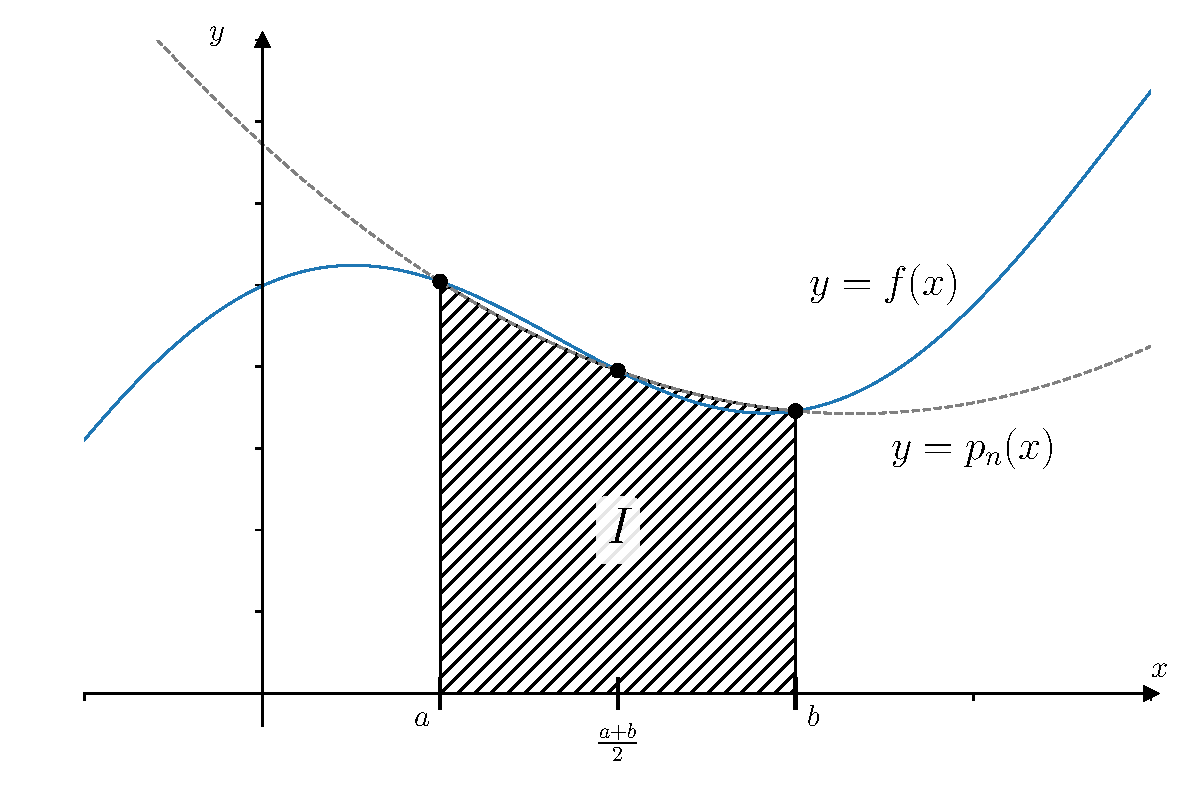
\includegraphics[width=0.6\textwidth]{figures/ch5_simpsons.pdf} 
	  \caption{.} \label{fig:ch5_simpsons}
	\end{center}
\end{figure}
The Newton-Cotes formula for $n=2$ is then
\begin{align*}
I \sim f(a) w_0 + f(\frac{a+b}{2}) w_1 + f(b) w_2.
\end{align*}
Let's derive expressions for the quadrature weights. Sometimes it will be convenient to use the midpoint $m=(a+b)/2$. Then the zeroth weight is
\begin{align*}
w_0 &= \int_a^b L_0(x) dx, \quad \text{and } L_0 = \frac{(x-m)(x-b)}{(a-m)(a-b)}.
\end{align*}
Let's integrate just the numerator for now
\begin{align*}
\int_a^b (x-m)(x-b) dx &= \left.\left( \frac{x^3}{3} - \frac{m+b}{2}x^2 + mbx \right) \right|_a^b \\
&=  \frac{b^3}{3} - \frac{m+b}{2}b^2 + mb^2  -  \frac{a^3}{3} + \frac{m+b}{2}a^2 - mba  \\
&=  \frac{b^3}{3} - \frac{ab^2}{4}  - \frac{b^3}{4} - \frac{b^3}{2} +  \frac{ab^2}{2} +  \frac{b^3}{2} -  \frac{a^3}{3} + \frac{a^3}{4} + \frac{ba^2}{4} + \frac{ba^2}{2} -  \frac{ba^2+ab^2}{2} \\
&= \frac{1}{12}\left(b^3 - 3ab^2 + 3ba^2 - a^3\right) \\
&= \frac{1}{12}\left(b - a\right)^3.
\end{align*}
The weight is then
\begin{align*}
w_0 &= \frac{1}{12} \frac{\left(b - a\right)^3}{(a-m)(a-b)} \\
 &= \frac{1}{12} \frac{\left(b - a\right)^2}{m-a}
\end{align*}
This denominator is
\begin{align*}
m-a = \frac{a+b}{2}-a = \frac{b-a}{2}
\end{align*}
and so the final expression for the weight is
\begin{align*}
w_0 = \frac{b-a}{6}.
\end{align*}
It's not so difficult to show that the other two weights are
\begin{align*}
w_1 &= \frac{4}{6}\left(b-a\right), \\
w_2 &= \frac{b-a}{6}.
\end{align*}
And so we have 

\noindent \fbox{\begin{minipage}{\linewidth}
\underline{\textbf{Simpson's rule for approximating an integral}}
\begin{align}
\int_a^b f(x)dx \sim \frac{b-a}{6}\left(f(a) + 4f\left(\frac{a+b}{2}\right)+ f(b) \right).
\end{align}
\end{minipage}}

Sometimes we use the distance between the interpolation points, $h=(b-a)/2$, and then Simpson's rule is written
\begin{align*}
\int_a^b f(x)dx \sim \frac{h}{3}\left(f(a) + 4f\left(\frac{a+b}{2}\right)+ f(b) \right).
\end{align*}
from which we get the alternative name \textit{Simpson's 1/3 rule}.

%%%%%%%%%%%%%%%%%%%%%%%%%%%%%%%%%%%%%%%%%%%%%%%
%%%%%%%%%%% EXAMPLE SIMPSON'S RULE %%%%%%%%%%%%
\exemple{\upline}
{
Integrate $f(x)=e^x$ from 0 to 4 using Simpson's rule with two (equal-sized) subdivisions.

\noindent The two subdivisions are the intervals $[0,2]$ and $[2,4]$. The areas are sketched out below
\begin{figure}[H]
	\begin{center}
	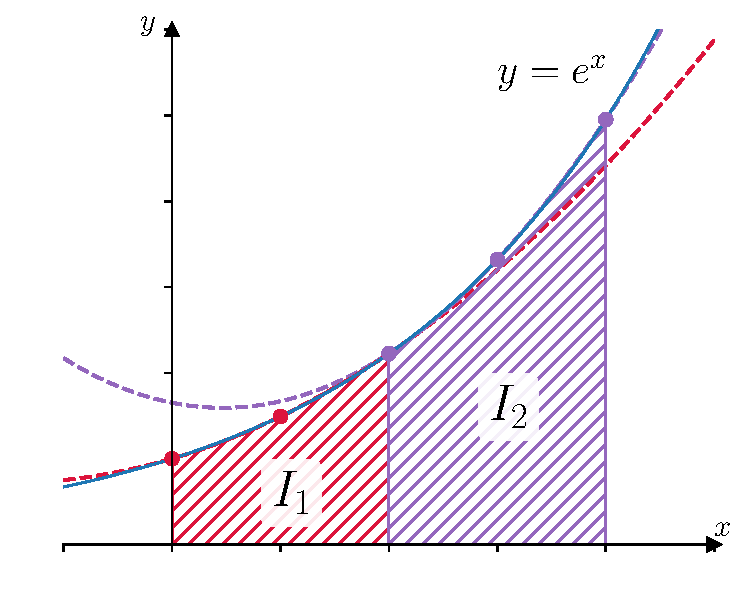
\includegraphics[width=0.6\textwidth]{figures/ch5_simpsons_example.pdf} 
	  \caption{.} \label{fig:ch5_simpsons_example}
	\end{center}
\end{figure}
\noindent The two integrals are then
\begin{align*}
&\int_0^2 e^x dx \sim I_1 = \frac{2-0}{6} \left(f(0) + 4f(1) + f(2) \right) = \frac{1}{3}\left(1 + 4e + e^2\right) \\
&\int_2^4 e^x dx \sim I_2 = \frac{4-2}{6} \left(f(2) + 4f(3) + f(4) \right) = \frac{1}{3}\left(e^2 + 4e^3 + e^4\right).
\end{align*}
Therefore the approximation of the total integral is just the addition of these two parts
\begin{align*}
\int_0^4 e^x dx \sim \frac{1}{3}\left(1 + 4e + 2e^2 + 4e^3 + e^4\right) \sim 53.9.
\end{align*}
This integral can be solved analytically for comparison
\begin{align*}
\int_0^4 e^x dx = \left. e^x\right|_0^4 = e^4 - 1 \sim 53.6.
\end{align*}
So the Simpson's rule approximation is much better than the Trapezium rule result.
}{\downline}
%%%%%%%%%%%%%%%%%%%%%%%%%%%%%%%%%%%%%%%%%%%%%%%
%%%%%%%%%%%%%%%%%%%%%%%%%%%%%%%%%%%%%%%%%%%%%%%


One final consideration: it's not necessarily the case that increasing the number of interpolation points increases the accuracy of the approximation. Consider the integral
\begin{align*}
\int_{-5}^5 \frac{1}{1+x^2} dx.
\end{align*}
Applying Newton-Cotes formulae with increasing $n$ does not converge, and in fact eventually increases without bound. It is generally better to stick with Simpson's rule, but to increase the number of subdivisions, as shown below:
\begin{figure}[H]
	\begin{center}
	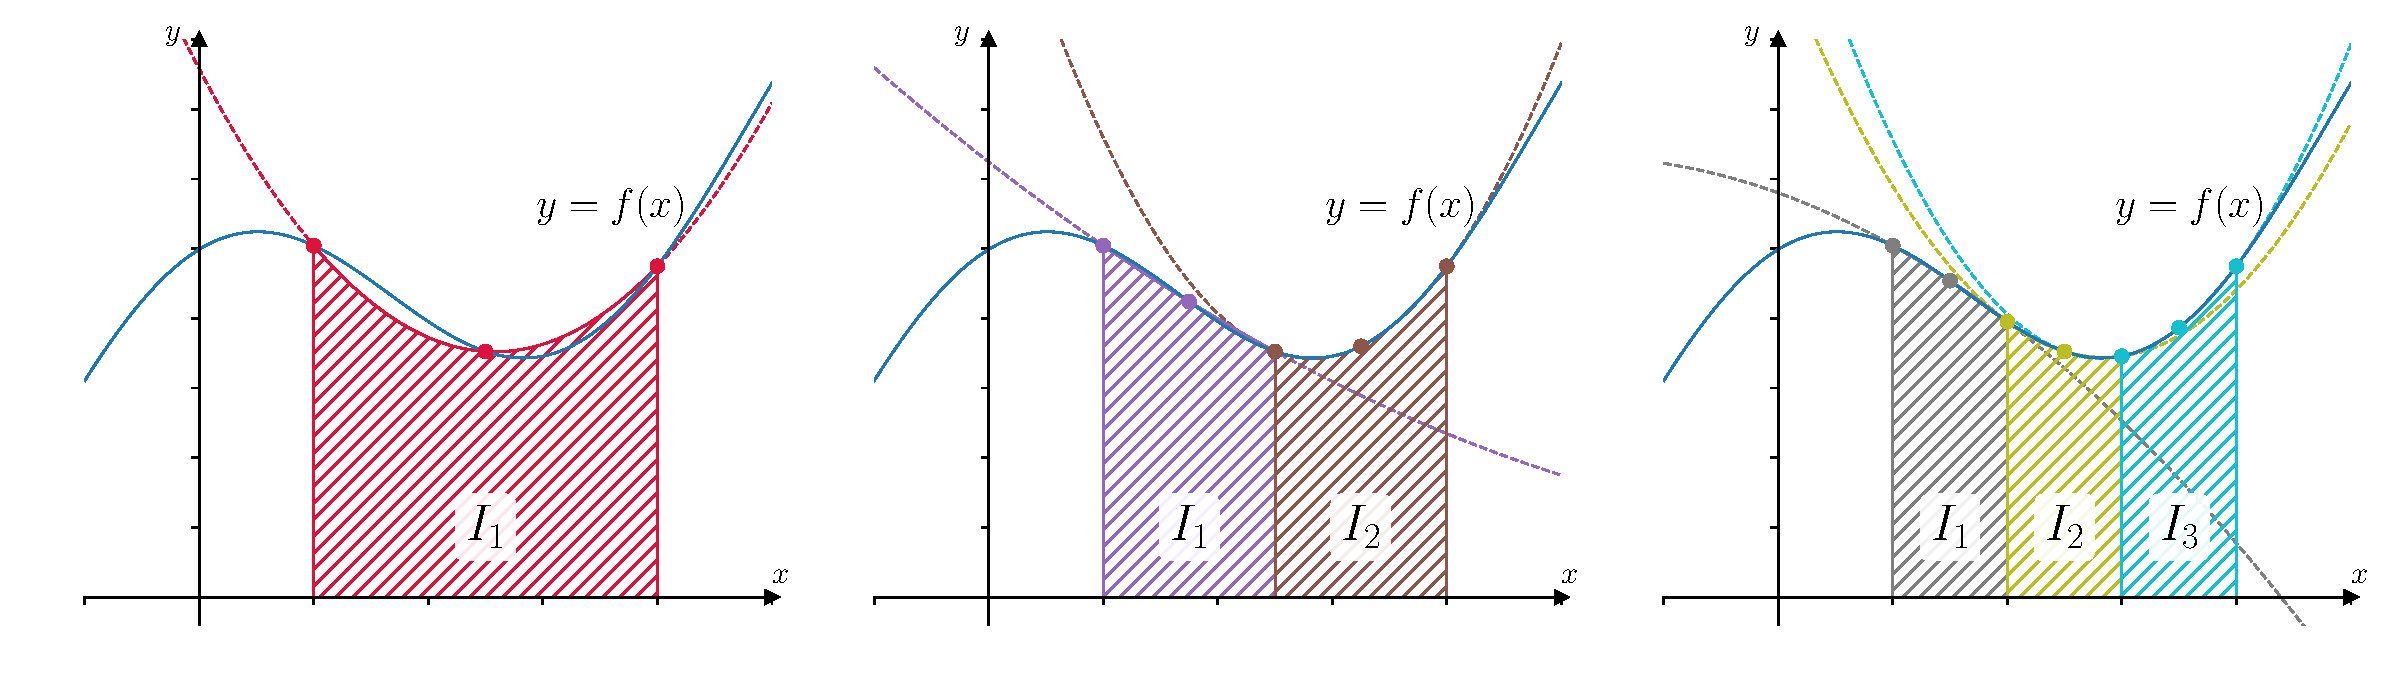
\includegraphics[width=\textwidth]{figures/ch5_simpsons_refinement.pdf} 
	  \caption{Simpson's rule using 1, 2 or 3 subdivisions.} \label{fig:ch5_simpsons_refinement}
	\end{center}
\end{figure}



\subsection{Degree of precision}

For an integration approximation scheme, the degree of precision of is the largest $k$ such that the integration scheme applied to $x^k$ gives the exact answer for $\int x^k \, dx$ which is of course $x^{k+1}/(k+1)$. That is, a scheme with degree of precision $k$ will be exact when applied to
\begin{align*}
1 \quad x \quad x^2 \quad \cdots \quad x^k
\end{align*}
but will fail to give the exact value when applied to $x^{k+1}$.

\exemple{\upline}{
Find the degree of precision for the Trapezium rule and for Simpson's rule. \\

\noindent For the Trapezium rule, when $f(x)=x^0$ we have
\begin{align*}
\int_a^b 1 dx \sim \frac{b-a}{2}\left(f(a) + f(b) \right) &= \frac{b-a}{2}\left(1 + 1 \right) \\
&= b-a \\
&= \left. x \right|_a^b
\end{align*}
This is exact so we check the next power. For $f(x)=x^1$ we have
\begin{align*}
\int_a^b x dx &\sim  \frac{b-a}{2}\left(a + b \right) \\
&= \frac{b^2-a^2}{2} \\
&= \left.\frac{x^2}{2} \right|_a^b
\end{align*}
This is exact so we check the next power. For $f(x)=x^2$ we have
\begin{align*}
\int_a^b x^2 dx &\sim \frac{b-a}{2}\left(a^2 + b^2 \right) \\
&= \frac{b^3 + ba^2 -ab^2 -a^3}{2} \\
& \neq \left.\frac{x^3}{3} \right|_a^b
\end{align*}
As $k=1$ is the highest power for which the Trapezium rule gave the exact result, the degree of precision is 1. \\

\noindent For Simpson's rule, when $f(x)=x^0$ we have
\begin{align*}
\int_a^b 1 dx \sim \frac{b-a}{6}\left(f(a) + 4f\left(\frac{a+b}{2}\right)+ f(b) \right)  &= \frac{b-a}{6}\left(1 + 4+ 1 \right). \\
&= b-a \\
&= \left. x \right|_a^b
\end{align*}
This is exact so we check the next power. For $f(x)=x^1$ we have
\begin{align*}
\int_a^b x dx &\sim \frac{b-a}{6}\left(a + 4\left(\frac{a+b}{2}\right)+ b \right)  \\
&= \frac{b-a}{6}\left(3a + 3b \right) \\
&= \frac{b^2-a^2}{2}\\
&= \left.\frac{x^2}{2} \right|_a^b
\end{align*}
This is exact so we check the next power. For $f(x)=x^2$ we have
\begin{align*}
\int_a^b x^2 dx &\sim \frac{b-a}{6}\left(a^2 + 4\left(\frac{a+b}{2}\right)^2+ b^2 \right)  \\
&= \frac{b-a}{6}\left(a^2 + 4\left(\frac{a^2+2ab + b^2}{4}\right)+ b^2 \right)  \\
&= \frac{b-a}{3}\left(a^2 +ab + b^2 \right) \\
&= \frac{b^3-a^3}{3} \\
&= \left.\frac{x^3}{3} \right|_a^b
\end{align*}
This is exact so we check the next power. For $f(x)=x^3$ we have
\begin{align*}
\int_a^b x^3 dx &\sim \frac{b-a}{6}\left(a^3 + 4\left(\frac{a+b}{2}\right)^3+ b^3 \right)  \\
&= \frac{b-a}{6}\left(a^3 + 4\left(\frac{a^3+3a^2b + 3ab^2  + b^3}{8}\right)+ b^3 \right)  \\
&= \frac{b-a}{6}\left(\frac{3}{2}a^3 + \frac{3}{2}a^2b + \frac{3}{2}ab^2+ \frac{3}{2}b^3 \right)  \\
&= \frac{b^4 - a^4}{4} \\
&= \left.\frac{x^4}{4} \right|_a^b
\end{align*}
This is exact so we check the next power. For $f(x)=x^4$ we have
\begin{align*}
\int_a^b x^4 dx &\sim \frac{b-a}{6}\left(a^4 + 4\left(\frac{a+b}{2}\right)^4+ b^4 \right)  \\
&= \frac{b-a}{6}\left(a^4 + 4\left(\frac{a^4 + 4 a^3 b + 6 a^2 b^2 + 4 a b^3  + b^4}{16}\right)+ b^4 \right)  \\
&= \frac{b-a}{24}\left(5 a^4 + 4 a^3 b + 6 a^2 b^2 + 4 a b^3  + 5 b^4 \right)  \\
&= \frac{5 b^5 + a^4 b - 2 a^3 b^2 + 2 a^2 b^3 - a b^4 - 5 a^5}{24}  \\
& \neq \left.\frac{x^5}{5} \right|_a^b
\end{align*}
As $k=3$ is the highest power for which Simpson's rule gave the exact result, the degree of precision is 3.
}{\downline}


%%%%%%%%%%%%%%%%%%%%%%%%%%%%%%%%%%%%%%%%%%
%%%%%%%%%%%%%%%%%%%%%%%%%%%%%%%%%%%%%%%%%%
%%%%%%%%%%%%%%%%%%%%%%%%%%%%%%%%%%%%%%%%%%








%%%%%%%%%%%%%%%%%%%%%%%%%%%%%%%%%%%%%%%%%%
%%%%%%%%%%%%%%%%%%%%%%%%%%%%%%%%%%%%%%%%%%
%%%%%%%%%%%%%%%%%%%%%%%%%%%%%%%%%%%%%%%%%%
%%%%%%%%%%%  DIFFERENTIATION %%%%%%%%%%%%%
%%%%%%%%%%%%%%%%%%%%%%%%%%%%%%%%%%%%%%%%%%
%%%%%%%%%%%%%%%%%%%%%%%%%%%%%%%%%%%%%%%%%%
%%%%%%%%%%%%%%%%%%%%%%%%%%%%%%%%%%%%%%%%%%
\section{Numerical differentiation}
The goal is to find the slope of some known function, $f(x)$, at a point $x=x_k$, giving just 1 real value
\begin{align*}
m=f'(x_k)
\end{align*}
as shown below.
\begin{figure}[H]
	\begin{center}
	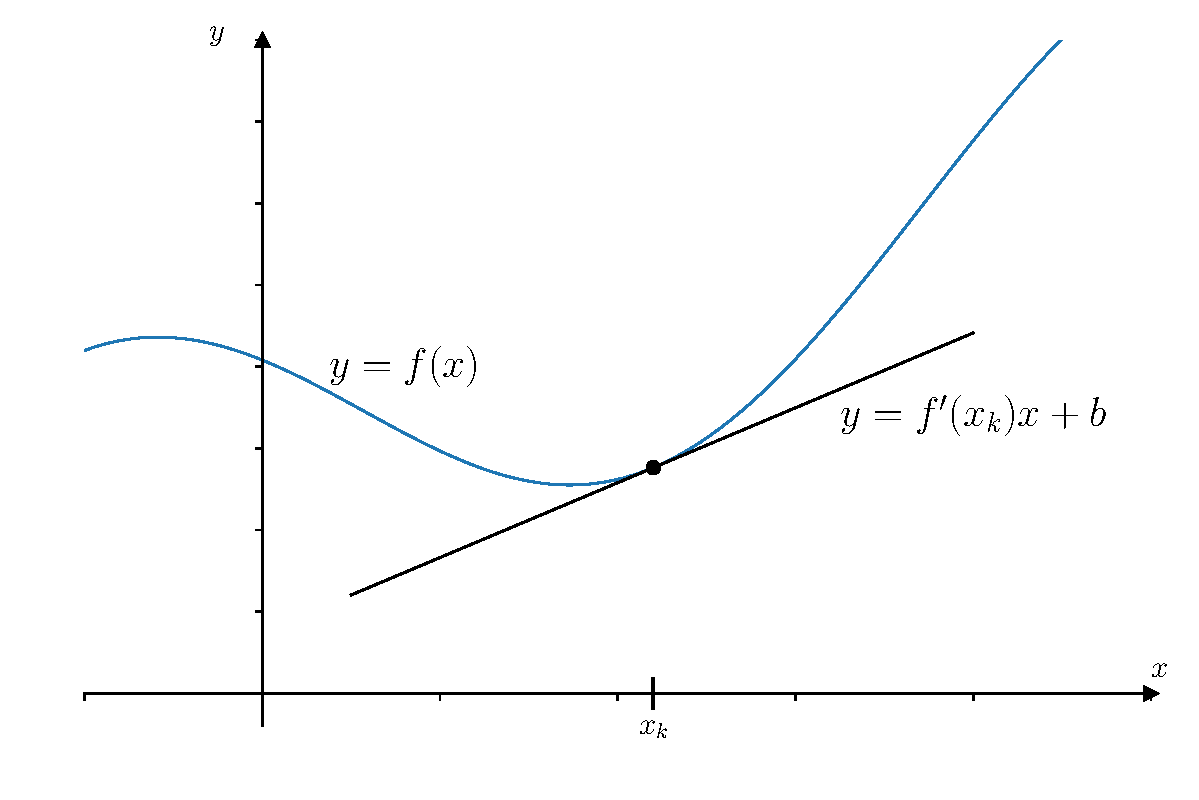
\includegraphics[width=0.6\textwidth]{figures/ch5_derivative.pdf} 
	  \caption{.} \label{fig:ch5_derivative}
	\end{center}
\end{figure}

The method will be just like with integration, we first estimate the function with a Lagrange polynomial, $p_n(x)$ and differentiate that instead (and then evaluate the polynomial at $x_k$)! That is,
\begin{align*}
f'(x_k) \sim \frac{d p_n}{dx}(x_k).
\end{align*}
We will here look at only $n=1$, which gives the forward and backward finite difference schemes, and $n=2$, which gives the centred finite difference scheme.

\subsection{Forward and backward finite difference}
For $n=1$, we need $n+1=2$ points of interpolation. Of course $x=x_k$ will be one of the points, but we have a free choice for the second point. If we choose the second point to be greater than $x_k$ we get the forward finite difference scheme, whereas if we choose it to be less than $x_k$ we get the backward finite difference scheme. The two schemes are illustrated below.
\begin{figure}[H]
	\begin{center}
	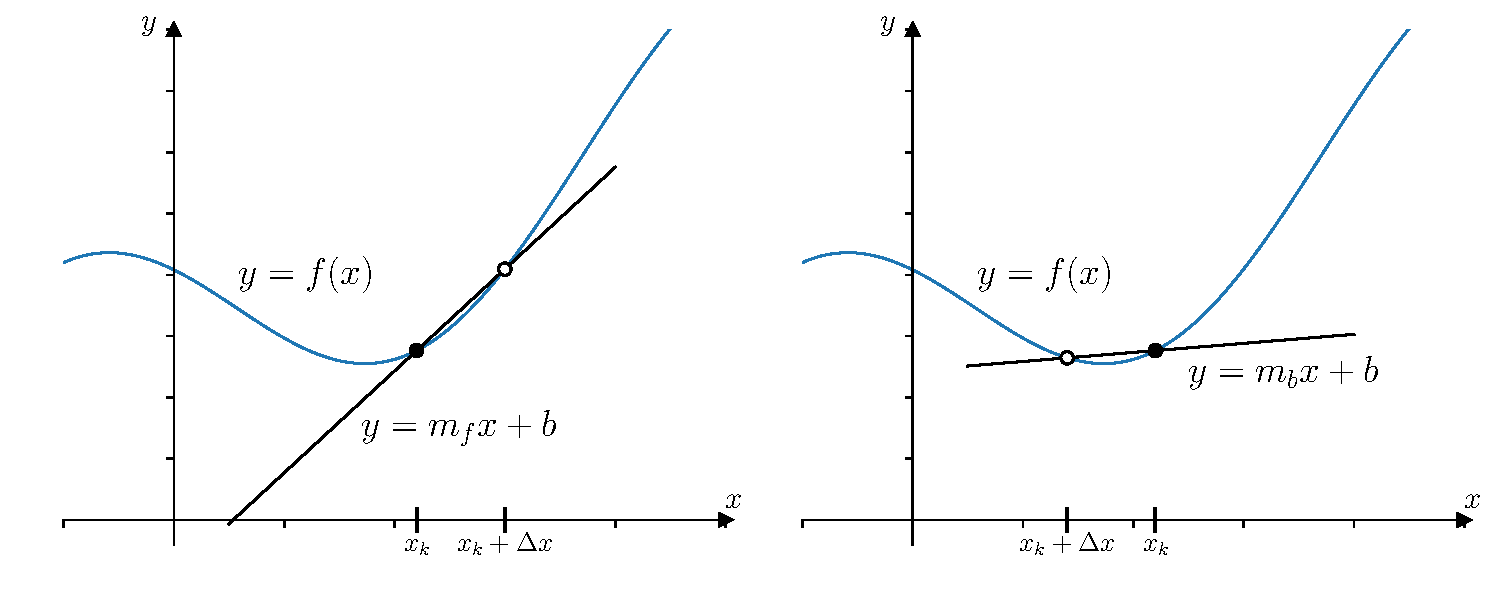
\includegraphics[width=\textwidth]{figures/ch5_forward_backward_difference.pdf} 
	  \caption{(Left) forward finite difference scheme and (right) backward finite difference scheme.} \label{fig:ch5_forward_backward_difference}
	\end{center}
\end{figure}
Consider the forward scheme, so that the interpolation positions are $x_0=x_k$ and $x_1=x_k+\Delta x$ for some small distance $\Delta x$. Then the Lagrange polynomial is given by
\begin{align*}
f(x) \sim p_1(x) = f(x_0) L_0(x) + f(x_1) L_1(x).
\end{align*}
The Lagrange basis polynomials are
\begin{align*}
L_0(x) &= \frac{x-x_1}{x_0-x_1} = \frac{x-x_k-\Delta x}{-\Delta x} \\
L_1(x) &= \frac{x-x_0}{x_1-x_0} = \frac{x-x_k}{\Delta x}.
\end{align*}
So the derivative of $f$ is approximated by
\begin{align*}
\frac{d p_1}{dx} &= f(x_0) \frac{dL_0}{dx} + f(x_1) \frac{dL_1}{dx} \\
 &= f(x_0) \frac{1}{-\Delta x} + f(x_1)\frac{1}{\Delta x} \\
 &= \frac{f(x_1)- f(x_0)}{\Delta x} \\
 &= \frac{f(x_k + \Delta x)- f(x_k)}{\Delta x}.
\end{align*}
I hope a sense of familiarity is tickling your brain right now, because this is exactly the form of the first principles definition of the derivative of a function at a point $x_k$
\begin{align*}
\frac{df}{dx}(x_k) = \lim_{\Delta x \to 0} \frac{f(x_k + \Delta x)- f(x_k)}{\Delta x}.
\end{align*}
So this scheme converges on the true derivative as $\Delta x$ becomes very small. So we have 

\vspace{0.2cm} \noindent \fbox{\begin{minipage}{\linewidth}
\underline{\textbf{Forward finite difference approximation of a derivative}}
\begin{align}
f'(x_k) \sim \frac{f(x_k + \Delta x)- f(x_k)}{\Delta x}.
\end{align}
\end{minipage}}\vspace{0.2cm} 

\noindent The formula for backward finite difference is quite straightforward (you should try to guess it before looking down)


\vspace{0.2cm} \noindent \fbox{\begin{minipage}{\linewidth}
\underline{\textbf{Backward finite difference approximation of a derivative}}
\begin{align}
f'(x_k) \sim \frac{f(x_k)- f(x_k - \Delta x)}{\Delta x}.
\end{align}
\end{minipage}}\vspace{0.2cm} 

The accuracy of these approximations can be assessed using the Taylor expansion of $f$
\begin{align*}
f(x) = \sum_{n=0}^{\infty} f^{(n)}(a)\frac{\left(x-a\right)^n}{n!}.
\end{align*}
We replace $x$ with $x+\Delta x$ and use $a=x$
\begin{align*}
f(x+\Delta x) &= \sum_{n=0}^{\infty} f^{(n)}(x)\frac{\left(\Delta x\right)^n}{n!} \\
&= f(x) + f'(x) \Delta x + f''(x) \frac{\left( \Delta x\right)^2}{2} + \cdots
\end{align*}
Rearranging for the first derivative
\begin{align*}
f'(x) = \underbrace{\frac{f(x+\Delta x) - f(x)}{\Delta x}}_{\text{forward finite difference scheme}} - \underbrace{f''(x) \frac{\Delta x}{2}}_\text{largest error term} - \cdots
\end{align*}
So we see that the largest error term is controlled by the second derivative (because further derivatives get multiplied by increasing powers of $\Delta x$, which becomes very small). This makes sense. Consider the graphs of the two functions below.
\begin{figure}[H]
	\begin{center}
	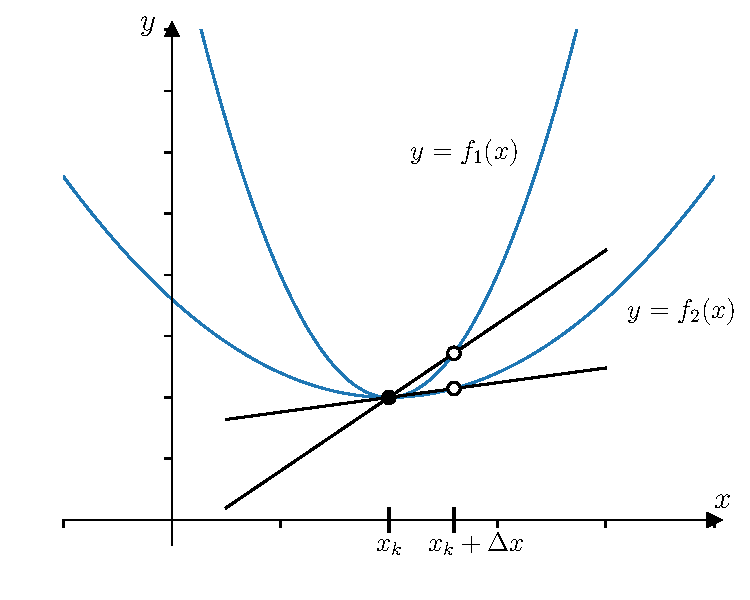
\includegraphics[width=0.8\textwidth]{figures/ch5_forward_difference_2nd_deriv.pdf} 
	  \caption{Two functions $f_1(x)$ and $f_2(x)$ with same first derivatives $f_1'(x_k)=f_2'(x_k)$ at $x=x_k$, but different second derivatives $f_1''(x_k)>f_2''(x_k)$.} \label{fig:ch5_forward_difference_2nd_deriv}
	\end{center}
\end{figure}
\noindent Both of these functions have the same slope at $x=x_k$. But the function $f_1(x)$ has a larger second derivative than $f_2(x)$ at that position. You can see that the forward finite difference approximation to the derivative at this position, despite using the same $\Delta x$, is worse for the function with larger second derivative at the position.

\exemple{\upline}{
Given the data
\begin{figure}[H]
\begin{tabular}{l|lllll}
$x$    & 4.5000   & 4.5025   & 4.5050   & 4.5075   & 4.5100 \\  \hline
$f(x)$ & 405.563  & 406.472  & 407.383  & 408.296  & 409.210
\end{tabular}
\end{figure}

\noindent Estimate estimate $f'(4.5050)$ by using forward finite difference with $\Delta x=0.0025$ and backward finite difference with $\Delta x=0.005$.

We are estimating the derivative at the position $x_k=4.5050$. For forward finite difference, $x_k+\Delta x=4.5075$. So we have
\begin{align*}
f'(4.5050) &= \frac{f(4.5075) - f(4.5050)}{0.0025} \\
&= \frac{408.296 - 407.383}{0.0025} \\
&\sim 365.200
\end{align*}

For backward finite difference with $\Delta x=0.005$ we have $x_k-\Delta x=4.5000$
\begin{align*}
f'(4.5050) &= \frac{f(4.5050) - f(4.5000)}{0.005} \\
&= \frac{407.383 - 405.563}{0.005} \\
&\sim 364.000
\end{align*}
}{\downline}





\subsection{Centred finite difference}
Now we consider $n=2$, so that we have $n+1=3$ interpolation points. The centred finite difference scheme uses the point of interest, at $x=x_k$, as one of the interpolation points, with the other two equidistant on either side, at $x=x_k \pm \Delta x$, as sketched below:
\begin{figure}[H]
	\begin{center}
	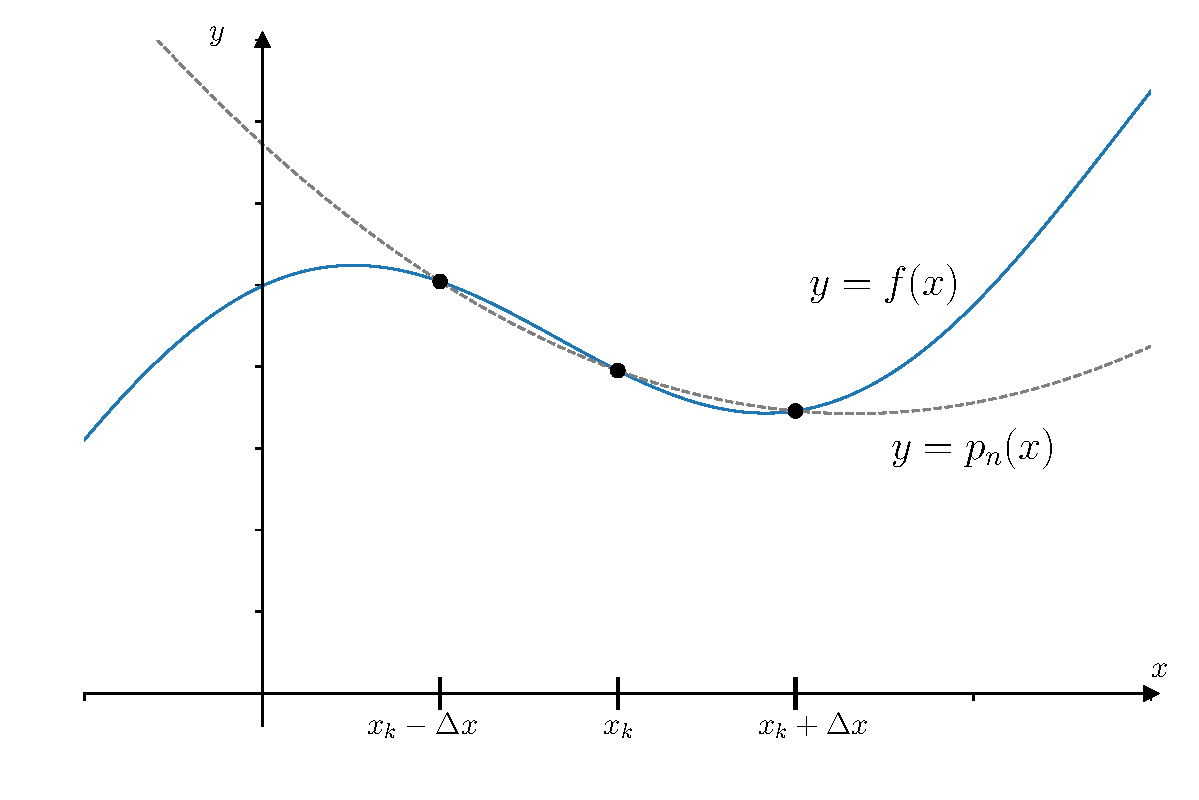
\includegraphics[width=0.6\textwidth]{figures/ch5_centred_finite_difference.pdf} 
	  \caption{Lagrange polynomial of order 2 (quadratic) used for the centred finite difference approximation to the derivative of $f(x)$ at $x=x_k$.} \label{fig:ch5_centred_finite_difference}
	\end{center}
\end{figure}
So, the Lagrange polynomial will be given by
\begin{align*}
f(x) \sim p_2(x) = f(x_k - \Delta x)L_0(x) + f(x_k)L_1(x) + f(x_k + \Delta x)L_2(x)
\end{align*}
Defining $x_0=x_k - \Delta x$, $x_1=x_k$ and  $x_2=x_k + \Delta x$, the basis polynomials are
\begin{align*}
L_0(x) &= \frac{(x-x_1)(x-x_2)}{(x_0-x_1)(x_0-x_2)} = \frac{x^2 - (x_1+x_2)x + x_1x_2}{(x_0-x_1)(x_0-x_2)} \\
%
L_1(x) &= \frac{(x-x_0)(x-x_2)}{(x_1-x_0)(x_1-x_2)} = \frac{x^2 - (x_0+x_2)x + x_0x_2}{(x_1-x_0)(x_1-x_2)} \\
%
L_2(x) &= \frac{(x-x_0)(x-x_1)}{(x_2-x_0)(x_2-x_1)} = \frac{x^2 - (x_0+x_1)x + x_0x_1}{(x_2-x_0)(x_2-x_1)}.
\end{align*}
As we will differentiate $p_2(x)$, we need the derivatives of these basis polynomials
\begin{align*}
L_0'(x) &= \frac{2x - (x_1+x_2)}{(x_0-x_1)(x_0-x_2)} = \frac{2x - 2x_k - \Delta x}{2(\Delta x)^2} \\
%
L_1'(x) &= \frac{2x - (x_0+x_2)}{(x_1-x_0)(x_1-x_2)} = \frac{2x - 2x_k}{-(\Delta x)^2}\\
%
L_2'(x) &= \frac{2x - (x_0+x_1)}{(x_2-x_0)(x_2-x_1)} = \frac{2x - 2x_k + \Delta x}{2(\Delta x)^2}.
\end{align*}
Then, we have the derivative of the Lagrange polynomial at the position $x=x_k$
\begin{align*}
\frac{dp_2}{dx}(x_k) &= f(x_k - \Delta x) L_0'(x_k) + f(x_k)L_1'(x_k) + f(x_k + \Delta x)L_2'(x_k) \\
&= \frac{-f(x_k - \Delta x) }{2\Delta x} + 0 +  \frac{+f(x_k + \Delta x) }{2\Delta x} 
\end{align*}
and so we get

\noindent \fbox{\begin{minipage}{\linewidth}
\underline{\textbf{Centred finite difference approximation of a derivative}}
\begin{align}
f'(x_k) \sim \frac{f(x_k + \Delta x)- f(x_k - \Delta x)}{2 \Delta x}.
\end{align}
\end{minipage}}

The three methods are summarised in one figure below
\begin{figure}[H]
	\begin{center}
	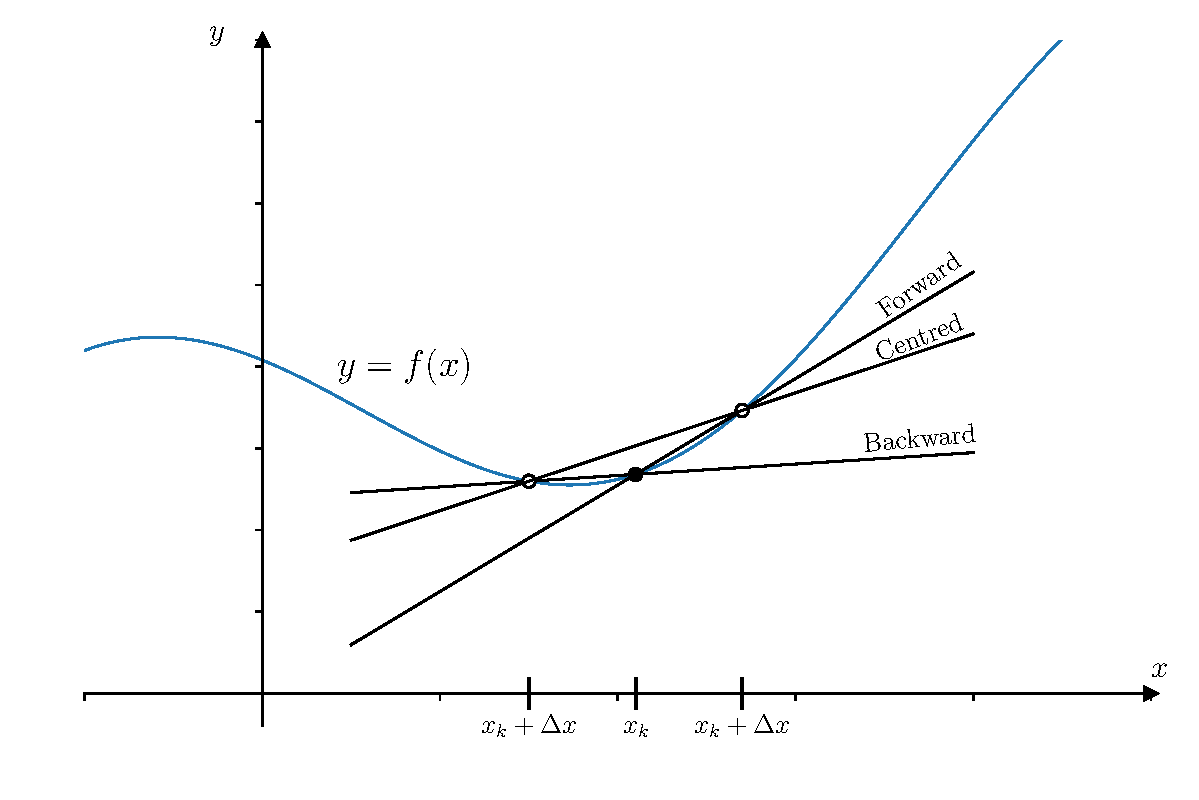
\includegraphics[width=0.9\textwidth]{figures/ch5_centred_forward_backward_difference.pdf} 
	  \caption{Forward, backward, and centred finite difference approximations to the derivative of $f(x)$ at the position $x=x_k$.} \label{fig:ch5_centred_forward_backward_difference}
	\end{center}
\end{figure}

What about the accuracy of the centred scheme? Let's go to the Taylor series again:
\begin{align*}
f(x+\Delta x) &= f(x) + f'(x) \Delta x + f''(x) \frac{\left( \Delta x\right)^2}{2} + f'''(x) \frac{\left( \Delta x\right)^3}{3!} + \cdots \\
f(x-\Delta x) &= f(x) - f'(x) \Delta x + f''(x) \frac{\left( \Delta x\right)^2}{2} - f'''(x) \frac{\left( \Delta x\right)^3}{3!} + \cdots
\end{align*}
Subtracting these two series removes the even terms
\begin{align*}
f(x+\Delta x) - f(x-\Delta x) = 2 f'(x) \Delta x + 2 f'''(x) \frac{\left( \Delta x\right)^3}{3!} + \cdots
\end{align*}
So, rearranging for the derivative gives
\begin{align*}
f'(x) = \frac{f(x+\Delta x) - f(x-\Delta x)}{2 \Delta x} - \underbrace{f'''(x) \frac{\left( \Delta x\right)^2}{3!}}_\text{largest error term} + \cdots
\end{align*}
This methoad has the \textit{third derivative} as the largest error term. So centred finite diffence is more accurate than backward or forward! We modeled the function with more Lagrange polynomial interpolation points, so it's good to be rewarded for that work.

We have analysed the accuracy of these three methods using Taylor expansions. When this is possible for a scheme we define the \textit{order of error} as power of the displacement $\Delta x$ in the largest error term. Hence the backward and forward finite difference schemes are first order schemes and the centred finite difference scheme is a second order scheme.

\exemple{\upline}{
Given the data
\begin{figure}[H]
\begin{tabular}{l|lllll}
$x$    & 4.5000   & 4.5025   & 4.5050   & 4.5075   & 4.5100 \\  \hline
$f(x)$ & 405.563  & 406.472  & 407.383  & 408.296  & 409.210
\end{tabular}
\end{figure}

\noindent Estimate estimate $f'(4.5050)$ by using centred finite difference with $\Delta x=0.0025$ and with $\Delta x=0.005$.

We are estimating the derivative at the position $x_k=4.5050$. For $\Delta x=0.0025$, the points we use are at $x=4.5025$ and $x=4.5075$. So we have
\begin{align*}
f'(4.5050) &= \frac{f(4.5075) - f(4.5025)}{2\times 0.0025} \\
&= \frac{408.296 - 406.472}{0.05} \\
&\sim 364.800
\end{align*}

For $\Delta x=0.005$, the points we use are at $x=4.5100$ and $x=4.5000$. So we have
\begin{align*}
f'(4.5050) &= \frac{f(4.5100) - f(4.5000)}{2\times 0.005} \\
&= \frac{409.210 - 405.563}{0.01} \\
&\sim 364.700
\end{align*}
}{\downline}




%%%%%%%%%%%%%%%%%%%%%%%%%%%%
%%%%%%%%%%%%%%%%%%%%%%%%%%%%
%%%%%%%%%%%%%%%%%%%%%%%%%%%%
%%%% Exercises %%%%
%%%%%%%%%%%%%%%%%%%%%%%%%%%%
%%%%%%%%%%%%%%%%%%%%%%%%%%%%
%%%%%%%%%%%%%%%%%%%%%%%%%%%%
\exercises{
\newpage
\section{Exercises}

\exercice{Given the function $f(x) = 2 \log(x+1)$}
\begin{enumerate}[label=\alph*)]
	\item Use the Trapezium rule to estimate the integral of $f(x)$ from [0,6] using 2 subdivisions.
	
	\item Use the Trapezium rule to estimate the integral of $f(x)$ from [0,6] using 3 subdivisions.
	
	\item Use Simpson's rule to estimate the integral of $f(x)$ from [0,6] using 2 subdivisions.
	
	\item Use Simpson's rule to estimate the integral of $f(x)$ from [0,6] using 3 subdivisions.
	
	\item Integrate $f(x)$ analytically to compare to the previous results.
\end{enumerate}


\exercice{Given the function $f(x) = 3 e^{0.5x} - 3$}
\begin{enumerate}[label=\alph*)]
	\item Use the Trapezium rule to estimate the integral of $f(x)$ from [0,6] using 2 subdivisions.
	
	\item Use the Trapezium rule to estimate the integral of $f(x)$ from [0,6] using 3 subdivisions.
	
	\item Use Simpson's rule to estimate the integral of $f(x)$ from [0,6] using 2 subdivisions.
	
	\item Use Simpson's rule to estimate the integral of $f(x)$ from [0,6] using 3 subdivisions.
	
	\item Integrate $f(x)$ analytically to compare to the previous results.
\end{enumerate}


\exercice{Given the function $f(x) = e^{\cos x}$}
\begin{enumerate}[label=\alph*)]
	\item Use the Trapezium rule to estimate the integral of $f(x)$ from $[0,2\pi]$ using 2 subdivisions.
	
	\item Use the Trapezium rule to estimate the integral of $f(x)$ from $[0,2\pi]$ using 3 subdivisions.
	
	\item Use Simpson's rule to estimate the integral of $f(x)$ from $[0,2\pi]$ using 2 subdivisions.
	
	\item Use Simpson's rule to estimate the integral of $f(x)$ from $[0,2\pi]$ using 3 subdivisions.
	
	\textit{Note: $f(x)$ cannot be integrated analytically (into elementary functions) to compare to the previous results.}
\end{enumerate}


\exercice{Given the data}
\begin{figure}[h]
\begin{tabular}{l|lllll}
$x$    & 2.0000   & 2.0025   & 2.0050   & 2.0075   & 2.0100 \\  \hline
$f(x)$ & 1.202604 & 1.214698 & 1.226929 & 1.239299 & 1.251809
\end{tabular}
\end{figure}

\begin{enumerate}[label=\alph*)]
	\item Use the forward finite difference scheme with h=0.005 to estimate $f'(2.005)$.
	
	\item Use the forward finite difference scheme with h=0.0025 to estimate $f'(2.005)$.

	\item Use the backward finite difference scheme with h=0.005 to estimate $f'(2.005)$.

	\item Use the backward finite difference scheme with h=0.0025 to estimate $f'(2.005)$.
	
	\item Use the centered finite difference scheme with h=0.005 to estimate $f'(2.005)$.

	\item Use the centered finite difference scheme with h=0.0025 to estimate $f'(2.005)$.

	\item The data were generated with $f(x)=\exp(x^2 + 10)/1000000$. What is the true derivative at $x=2.005$?
\end{enumerate}


\exercice{Given the data}
\begin{figure}[h]
\begin{tabular}{l|lllll}
$x$    & 7.5000   & 7.5025   & 7.5050   & 7.5075   & 7.5100 \\  \hline
$f(x)$ & 384.375 & 384.785 & 385.194 & 385.604 & 386.015
\end{tabular}
\end{figure}          

\begin{enumerate}[label=\alph*)]
	\item Use the forward finite difference scheme with h=0.005 to estimate $f'(7.505)$.
	
	\item Use the forward finite difference scheme with h=0.0025 to estimate $f'(7.505)$.

	\item Use the backward finite difference scheme with h=0.005 to estimate $f'(7.505)$.

	\item Use the backward finite difference scheme with h=0.0025 to estimate $f'(7.505)$.
	
	\item Use the centered finite difference scheme with h=0.005 to estimate $f'(7.505)$.

	\item Use the centered finite difference scheme with h=0.0025 to estimate $f'(7.505)$.

	\item The data were generated with $f(x)=x^3 - 5x$. What is the true derivative at $x=7.505$?
\end{enumerate}


\exercice{Given the data}
\begin{figure}[h]
\begin{tabular}{l|lllll}
$x$    & 1.560   & 1.561   & 1.562   & 1.563   & 1.564 \\  \hline
$f(x)$ & 92.6204 & 102.076 & 113.681 & 128.263 & 147.136
\end{tabular}
\end{figure}

\begin{enumerate}[label=\alph*)]
	\item Use the forward finite difference scheme with h=0.002 to estimate $f'(1.562)$.
	
	\item Use the forward finite difference scheme with h=0.001 to estimate $f'(1.562)$.

	\item Use the backward finite difference scheme with h=0.002 to estimate $f'(1.562)$.

	\item Use the backward finite difference scheme with h=0.001 to estimate $f'(1.562)$.
	
	\item Use the centered finite difference scheme with h=0.002 to estimate $f'(1.562)$.

	\item Use the centered finite difference scheme with h=0.001 to estimate $f'(1.562)$.

	\item The data were generated with $f(x)=\tan x$. What is the true derivative at $x=7.505$?
\end{enumerate}

}

